
% Asset ID: A21RadiansTikZ-003
% Purpose: Show sine and cosine graphs with radian-labelled axes.
\documentclass[tikz,border=8pt]{standalone}
\usepackage{pgfplots}
\pgfplotsset{compat=1.18}
\begin{document}
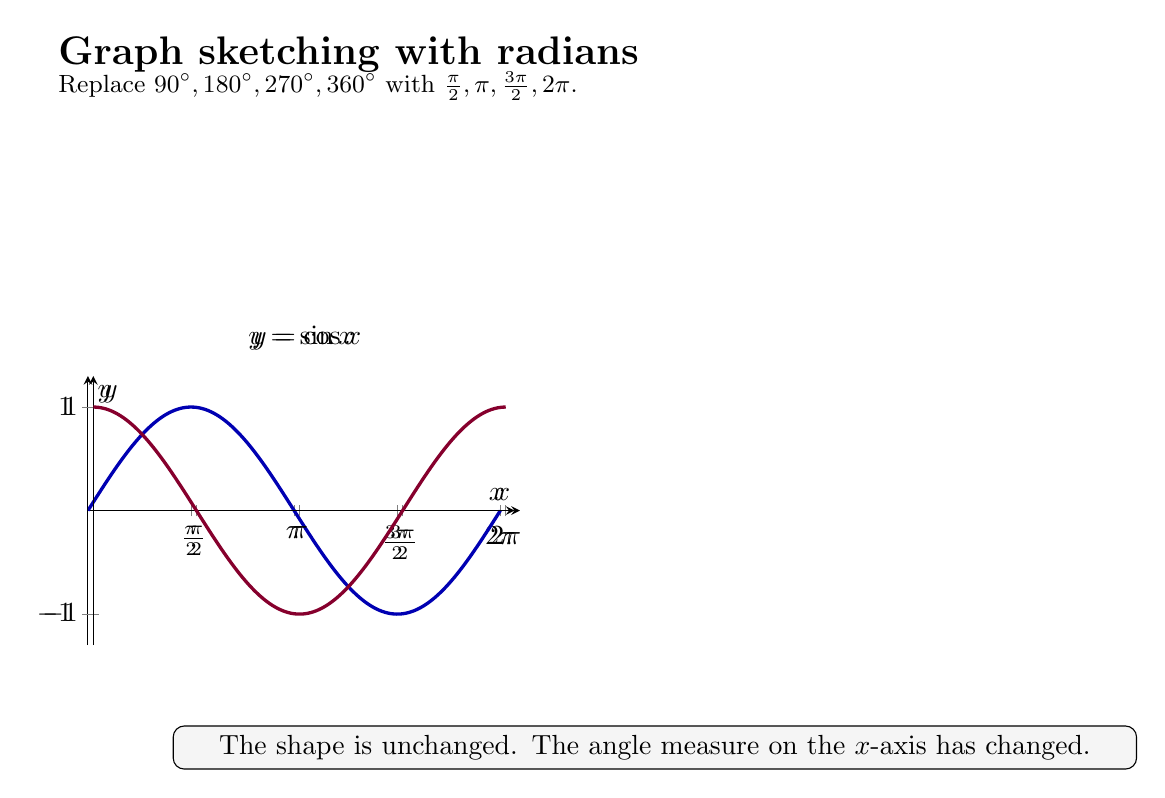
\begin{tikzpicture}
\node[anchor=west,font=\bfseries\Large] at (-0.5,7.5) {Graph sketching with radians};
\node[anchor=west,font=\small] at (-0.5,7.1) {Replace \(90^\circ,180^\circ,270^\circ,360^\circ\) with \(\frac{\pi}{2},\pi,\frac{3\pi}{2},2\pi\).};
\begin{axis}[at={(0,0)},width=7cm,height=5cm,axis lines=middle,xmin=0,xmax=6.5,ymin=-1.3,ymax=1.3,xtick={1.5708,3.1416,4.7124,6.2832},xticklabels={\(\frac{\pi}{2}\),\(\pi\),\(\frac{3\pi}{2}\),\(2\pi\)},ytick={-1,1},yticklabels={\(-1\),\(1\)},xlabel={\(x\)},ylabel={\(y\)},title={\(y=\sin x\)},samples=200,domain=0:6.2832]
\addplot[very thick,blue!70!black] {sin(deg(x))};
\end{axis}
\begin{axis}[at={(8.2,0)},width=7cm,height=5cm,axis lines=middle,xmin=0,xmax=6.5,ymin=-1.3,ymax=1.3,xtick={1.5708,3.1416,4.7124,6.2832},xticklabels={\(\frac{\pi}{2}\),\(\pi\),\(\frac{3\pi}{2}\),\(2\pi\)},ytick={-1,1},yticklabels={\(-1\),\(1\)},xlabel={\(x\)},ylabel={\(y\)},title={\(y=\cos x\)},samples=200,domain=0:6.2832]
\addplot[very thick,purple!70!black] {cos(deg(x))};
\end{axis}
\node[draw,rounded corners,fill=gray!8,align=center,text width=12cm] at (7.2,-1.3) {The shape is unchanged. The angle measure on the \(x\)-axis has changed.};
\end{tikzpicture}
\end{document}
